\documentclass[a4paper,11pt]{article}
\usepackage{cmap}
\usepackage{polski}
\usepackage[T1]{fontenc}
\usepackage[utf8]{inputenc}
\usepackage{graphicx}
\usepackage{minted}
\usepackage{titlesec}

\titlelabel{\thetitle.\quad}

\date{
{Data zajęć: --- \hfill Data oddania: 28.01.2019}
\\
{Termin zajęć: Pon. TP 9:15\hfill Prowadzący zajęcia: Mgr inż. Szymon Datko}
}
\title{Sprawozdanie nr 6 - Projekt}
\author{Jakub Majewski 238902}

\makeatletter
\renewcommand{\maketitle}{
   \begin{titlepage}
     \begin{center}
       {\@date}
       \\
       \par\vspace{3ex}
       {\LARGE\@title}
       \par\vspace{1ex}
       \begin{tabular}[t]{c}
         \@author
       \end{tabular}
     \end{center}
     \@thanks
   \end{titlepage}
}
\makeatother

\begin{document}

\begin{center}\Large
    Grafika Komputerowa i Komunikacja Człowiek-Komputer
\end{center}

\hrule
    {\let\newpage\relax\maketitle}
\hrule
 
% ******************************* OPIS TEMATU *******************************

\section{Opis tematu}

Temat: Renderowanie obiektów 2D i 3D w przeglądarce z użyciem biblioteki WebGL. \\ \\
Zrealizowane zadania: \\
1. wyrenderowanie obiektu 2D z użyciem obiektu 'canvas', \\
2. wyrenderowanie obiektu 3D w kształcie sześciennego pudełka, \\
3. nałożenie tekstury na wyrenderowany obiekt 3D, \\
4. wyrenderowanie oteksturowanego czworościanu foremnego, \\
5. wyrenderowanie dywanu Sierpińskiego w 3D (kostki Sierpińskiego).

% ******************************* OPIS NAJWAŻNIEJSZYCH FRAGMENTÓW KODU *******************************

\newpage
\section{Opis najważniejszych fragmentów kodu}

\noindent 1. Tworzenie obiektu typu 'canvas' w pliku .html.
\begin{minted}[linenos,tabsize=2,breaklines]{HTML}
<body>
	<!-- ... -->
	<canvas id="glcanvas" width="500" height="500" style="border: 1px solid #66666D; background-color: #545469;">
		Brak wsparcia dla elementu HTML5 typu canvas 
	</canvas>
	<!-- ... -->
</body>
\end{minted}

\noindent 2. Inicjalizacja parametrów WebGL, shaderów oraz tablic wierzchołków \\i ścian renderowanych obiektów.
\begin{minted}[linenos,tabsize=2,breaklines]{JS}
function runWebGL () {
	gl_canvas = document.getElementById("glcanvas");
	gl_ctx = gl_getContext(gl_canvas);    
	gl_initShaders();
	gl_initBuffers();
	gl_setMatrix();    
	gl_draw(); 
}
\end{minted}
\newpage

\noindent 3. Przykładowy shader wierzchołków w języku GLSL.
\begin{minted}[linenos,tabsize=2,breaklines]{GLSL}
	attribute vec3 position;
	attribute vec3 color;

	uniform mat4 PosMatrix;
	uniform mat4 MovMatrix;
	uniform mat4 ViewMatrix;
	uniform float u_timev;

	varying vec3 vColor;
	
	void main(void) {
		gl_Position = PosMatrix * ViewMatrix * MovMatrix * vec4(position, 1.);
		gl_Position.x += 0.25 * cos(4.0*u_timev);
		gl_Position.y += 0.25 * sin(4.0*u_timev);
		vColor = color;
	}
\end{minted}
\newpage

\noindent 4. Przykładowy shader fragmentów w języku GLSL.
\begin{minted}[linenos,tabsize=2,breaklines]{GLSL}
	precision mediump float;

	uniform float u_time;

	varying vec3 vColor;
	
	vec3 rgb2hsv(vec3 c) {
	    vec4 K = vec4(0.0, -1.0 / 3.0, 2.0 / 3.0, -1.0);
	    vec4 p = mix(vec4(c.bg, K.wz), vec4(c.gb, K.xy), step(c.b, c.g));
	    vec4 q = mix(vec4(p.xyw, c.r), vec4(c.r, p.yzx), step(p.x, c.r));
	
	    float d = q.x - min(q.w, q.y);
	    float e = 1.0e-10;
	    return vec3(abs(q.z + (q.w - q.y) / (6.0 * d + e)), d / (q.x + e), q.x);
	}
	
	vec3 hsv2rgb(vec3 c) {
	    vec4 K = vec4(1.0, 2.0 / 3.0, 1.0 / 3.0, 3.0);
	    vec3 p = abs(fract(c.xxx + K.xyz) * 6.0 - K.www);
	    return c.z * mix(K.xxx, clamp(p - K.xxx, 0.0, 1.0), c.y);
	}
	
	void main(void) {
		vec3 hsv = rgb2hsv(vColor);
		hsv.r += abs(sin(u_time)); 
		vec3 col = hsv2rgb(hsv);
		gl_FragColor = vec4(col, 1.);
	}
\end{minted}
\newpage

\noindent 5. Funkcje odpowiedzialne za inicjalizację shaderów i załączenia ich do aplikacji.
\begin{minted}[linenos,tabsize=2,breaklines]{JS}

// Funkcja tworząca nowy shader
function getShader(source, type, typeString) {       
	var shader = gl_ctx.createShader(type);       
	gl_ctx.shaderSource(shader, source);
	gl_ctx.compileShader(shader);        
	if (!gl_ctx.getShaderParameter(shader, gl_ctx.COMPILE_STATUS)) {
		alert('error in' + typeString);          
		return false;
	}
	return shader;    
};

// Funkcja inicjalizująca i załączająca shadery
function gl_initShaders () {
	var vsCode = "..."; // Kod shadera wierzchołków
	var fsCode = "..."; // Kod shadera fragmentów 
	var shaderProgram = gl_ctx.createProgram();    

	// Tworznie pojedynczych shaderów i łączenie ich w jeden duży
	gl_ctx.attachShader(shaderProgram, getShader(vsCode, gl_ctx.VERTEX_SHADER, "VERTEX"));
	gl_ctx.attachShader(shaderProgram, getShader(fsCode, gl_ctx.FRAGMENT_SHADER, "FRAGMENT"));     
	gl_ctx.linkProgram(shaderProgram);     

	// Tworzenie nowych uniformów oraz referencji do nich
	_uniformMyPos = gl_ctx.getUniformLocation(shaderProgram, "my_pos");    
	//... reszta atrybutów

	// Tworzenie nowych atrybutów oraz referencji do nich
	_attrPosition = gl_ctx.getAttribLocation(shaderProgram, "position");  
	gl_ctx.enableVertexAttribArray(_position);   
	//... reszta atrybutów

	// Załączenie skonfigurowanego shadera do silnika WebGL
	gl_ctx.useProgram(shaderProgram); 
} 
\end{minted}
\newpage

\noindent 6. Funkcje tworzące tablice wierzchołków i ścian obiektu o kształcie sześcianu.
\begin{minted}[linenos,tabsize=2,breaklines]{JS}

function defineCubeVertices(x, y, z, size) {
	var xs = x+size;
	var ys = y+size;
	var zs = z+size;
	var vertices = [
		// Bottom
		x,y,zs,		0,0,0,
		x,y,z,		0,0,1,
		xs,y,z,		0,1,0,
		xs,y,zs,	0,1,1,
		// Top
		x,ys,zs,	1,0,0,
		x,ys,z,		1,0,1,
		xs,ys,z,	1,1,0,
		xs,ys,zs,	1,1,1,
	];
	return vertices;
}

function defineCubeFaces(firstVertexIdx) {
	var faces = [
	   4, 7, 6, 6, 5, 4, // Top wall
	   0, 1, 5, 5, 4, 0, // Left
	   1, 2, 6, 6, 5, 1, // Back
	   2, 3, 7, 7, 6, 2, // Right
	   0, 3, 7, 7, 4, 0, // Front
	   0, 1, 2, 2, 3, 0, // Bottom
	];

	for (var i = faces.length - 1; i >= 0; i--) {
		faces[i] += firstVertexIdx;
	}

	return faces;
}

\end{minted}
\newpage

\noindent 7. Funkcje odpowiadające za stworzenie tablicy wierzchołków oraz ścian dla kostki Sierpińskiego o podanej wielkości i poziomie rekurencji.
\begin{minted}[linenos,tabsize=2,breaklines]{JS}

SIERPINSKI_FILLED_CUBES = [[0,0,0], [1,0,0], [2,0,0], [0,1,0], [2,1,0], [0,2,0], [1,2,0], [2,2,0],	[0,0,1], [2,0,1], [0,2,1], [2,2,1],	[0,0,2], [1,0,2], [2,0,2], [0,1,2], [2,1,2], [0,2,2], [1,2,2], [2,2,2]];

function rSierpinski(x, y, z, size, lvl, maxLvl, vertices, faces) {
	if (lvl != maxLvl) {
		size = size / 3;		
		SIERPINSKI_FILLED_CUBES.forEach(function(vec){
			rSierpinski(x+size*vec[0], y+size*vec[1], z+size*vec[2], size, lvl+1, maxLvl, vertices, faces);
		});
	}
	else {
		var newFaces = defineCubeFaces(vertices.value.length / 6);
		var newVertices = defineCubeVertices(x, y, z, size);

		newVertices.forEach(function(vertex) { vertices.value.push(vertex); });
		newFaces.forEach(function(face) { faces.value.push(face); });
	}
}

function sierpinski(size, n) {
	var xyz = -size/2;
	var vertices = {value: []};
	var faces = {value: []};

	if(n == 0) {
		vertices.value = defineCubeVertices(xyz,xyz,xyz,size);
		faces.value = defineCubeFaces(0);
	}
	else {
		rSierpinski(xyz, xyz, xyz, size, 0, n, vertices, faces);
	}
	return {
		vertices: vertices.value, faces: faces.value
	};
}
\end{minted}
\newpage

\noindent 8. Funkcja inicjalizująca wyświetlanie oraz głowna pętla renderowania.
\begin{minted}[linenos,tabsize=2,breaklines]{JS}
function gl_draw() {    
	gl_ctx.clearColor(0.0, 0.0, 0.0, 0.0);    
	gl_ctx.enable(gl_ctx.DEPTH_TEST);    
	gl_ctx.depthFunc(gl_ctx.LEQUAL);    
	gl_ctx.clearDepth(1.0);   
	var timeOld = 0;     

	// Funkcja pełniąca rolę pętli renderowania
	var animate = function (time) {       
		var dAngle = rotationSpeed * (time - timeOld);  
		timeOld = time;        

		if (X) MATRIX.rotateX(_matrixMovement, dAngle);
		if (Y) MATRIX.rotateY(_matrixMovement, dAngle);
		if (Z) MATRIX.rotateZ(_matrixMovement, dAngle);

		gl_ctx.viewport(0.0, 0.0, gl_canvas.width, gl_canvas.height);
		gl_ctx.clear(gl_ctx.COLOR_BUFFER_BIT | gl_ctx.DEPTH_BUFFER_BIT);        

		// Nadawanie wartości uniformom w shaderach
		gl_ctx.uniformMatrix4fv(_uniformMat4, false, mat4Value);    
		gl_ctx.uniform1f(_uniformFloat, floatValue);
		//...

		// Ustawienie dla atrybutu referencji do pozycji wierzchołka w shaderze
		gl_ctx.vertexAttribPointer(_attrPosition, 3, gl_ctx.FLOAT, false, 4*(3+3), 0);  
		//...

		gl_ctx.bindBuffer(gl_ctx.ARRAY_BUFFER, _verticesBuffer);       
		gl_ctx.bindBuffer(gl_ctx.ELEMENT_ARRAY_BUFFER, _facesBuffer);     
		gl_ctx.drawElements(gl_ctx.TRIANGLES, faces.length, gl_ctx.UNSIGNED_SHORT, 0); 
		gl_ctx.flush();        
		window.requestAnimationFrame(animate);    
	};    
	animate(0); 
}
\end{minted}
\newpage

% ******************************* REZULTAT PRACY *******************************

\section{Rezultat pracy}

\begin{figure}[h!]
    \centering
    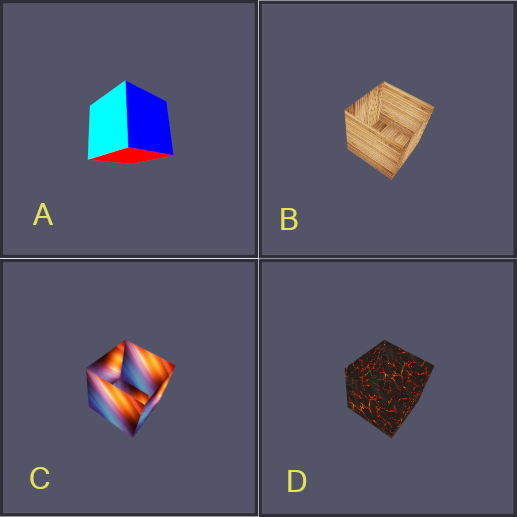
\includegraphics[width=1.0\linewidth]{cube.png}
    \caption{Kostka z kolorowymi ścianami (A), oraz pudełko z nałożoną teksturą (B)(C)(D).}
    \label{fig:pic1}
\end{figure}
\newpage

\begin{figure}[h!]
    \centering
    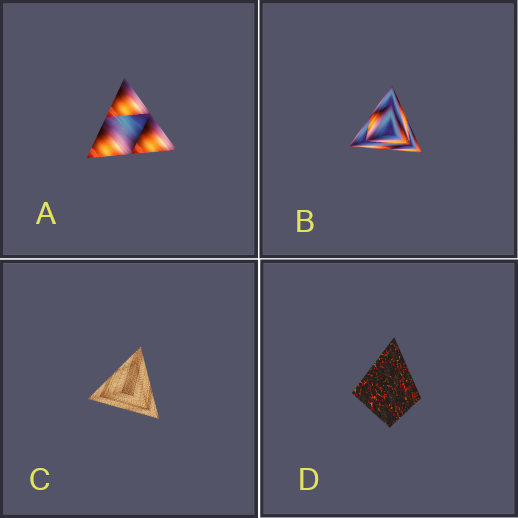
\includegraphics[width=1.0\linewidth]{tetra.png}
    \caption{Czworościan foremny z nałożoną teksturą obserwowany od boku (A)(D) oraz z góry (B)(C).}
    \label{fig:pic2}
\end{figure}
\newpage

\begin{figure}[h!]
    \centering
    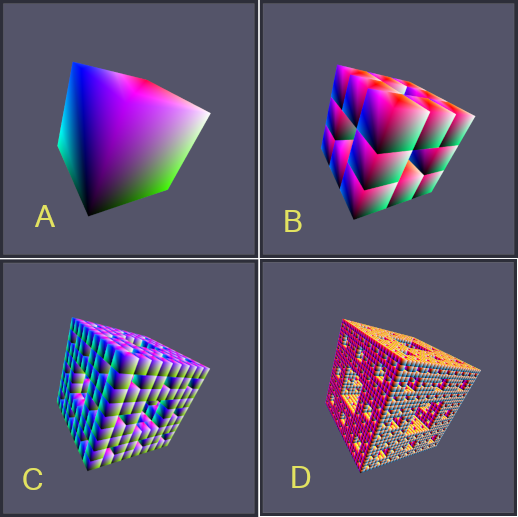
\includegraphics[width=1.0\linewidth]{sierp.png}
    \caption{Dywan sierpińskiego wyrenderowany w 3D o poziomie rekurencji równym kolejno: 0 (A), 1 (B), 2 (C) i 3 (D).}
    \label{fig:pic3}
\end{figure}
\newpage

\newpage

% ******************************* SPOSTRZEŻENIA I WNIOSKI *******************************

\section{Spostrzeżenia i wnioski}
Podczas wykonywania ćwiczenia znacznie rozwinąłem swoją wiedzę nie tylko w zakresie renderowania obiektów z użyciem biblioteki WebGL, ale również dowiedziałem się m.in. jak łączyć ze sobą frontend i backend na stronach internetowych. W realizacji zadania zastosowałem autorski algorytm generowania dywanu Sierpińskiego w 3D bazując na podstawie przygotowanych wcześniej konceptów. Na początku nie był on wystarczająco szybki. Implementacja algorytmu przeszła ok. 4 duże zmiany, tylko i wyłącznie w celach optymalizacyjnych. Pierwsza wersja implementacji powodowała kilkusekundowe opóźnienie ładowania się strony już na generowaniu kostki o poziomie rekurencji równym 2.

\end{document}